\chapter{LND instrument}
\label{chp:LNDinstrument}

This supplement chapter provides the simulation setup of \ac{LND}, the overview of the \ac{LND} measurements in the last four years (2019 - 2023) and several potential topic that worth to be investigated in the future.

\section{LND simulation set-up}
\label{chp:LNDsimulation}

As explained by \citet{Wimmer-2020-LND}, the response of the \ac{LND} to energetic particles is decided by both experimental calibration in the laboratory and the simulation in the \ac{Geant4} toolkit. This section we mainly explain the simulation setup of \ac{LND}.

Fig.~\ref{fig:LND_simulation_model}
show a screenshot of the \ac{LND} simulation model that we utilized in the \ac{Geant4} simulation. The construction of this model is based on the computer-aided design (CAD) and initially finished by Henning Lohf. 
The outermost lines define the world of the simulation which is 20cm $\times$ 20cm $\times$ 20cm. The space inside of the box is filled with vaccume. The smaller-size but complicated structures in white color in the center is the housing of the \ac{LND} sensor head, which is composed of several Al board.
The olive colored layers in the sensor head are the carriers that support the \acp{SSD} which are in the blue color. The pink color represent the Gd foils which are used to detect the thermal neutrons. In the end, the two green slab are the printed circuit board.


\begin{figure}[!htb]
    \centering
    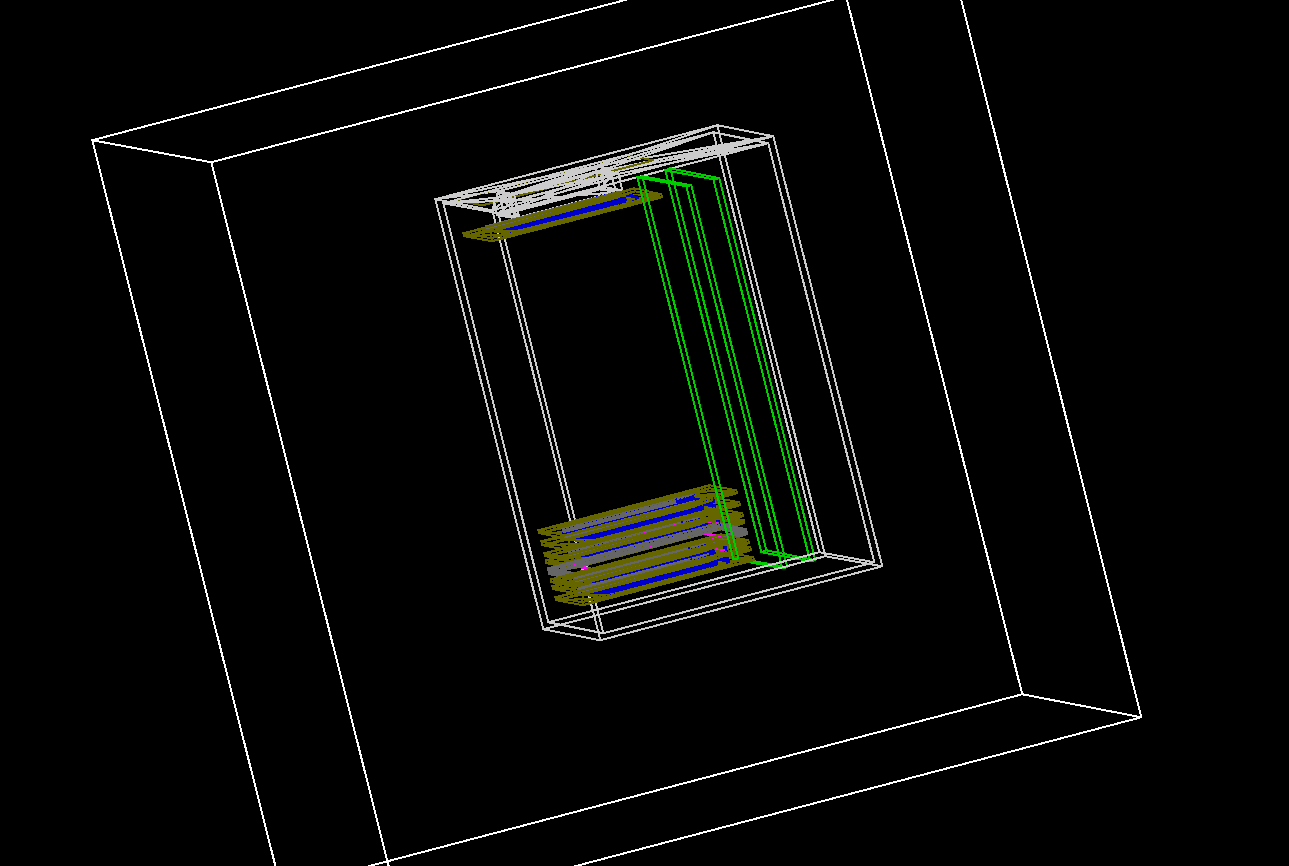
\includegraphics[width= 0.89\textwidth, height = 0.6\textwidth]{images/LND_model.png}
    \caption[The sketch of \ac{LND} sensor head]{The sketch structure of the \ac{LND} sensor head that is utilized in the \ac{Geant4} simultion. The sizes of each piece of structures are take from the CAD model of \ac{LND}}
    \label{fig:LND_simulation_model}
\end{figure}


\section{The overall proton, helium and TID variation and the most updated SEP list}

\begin{figure}
    \centering
    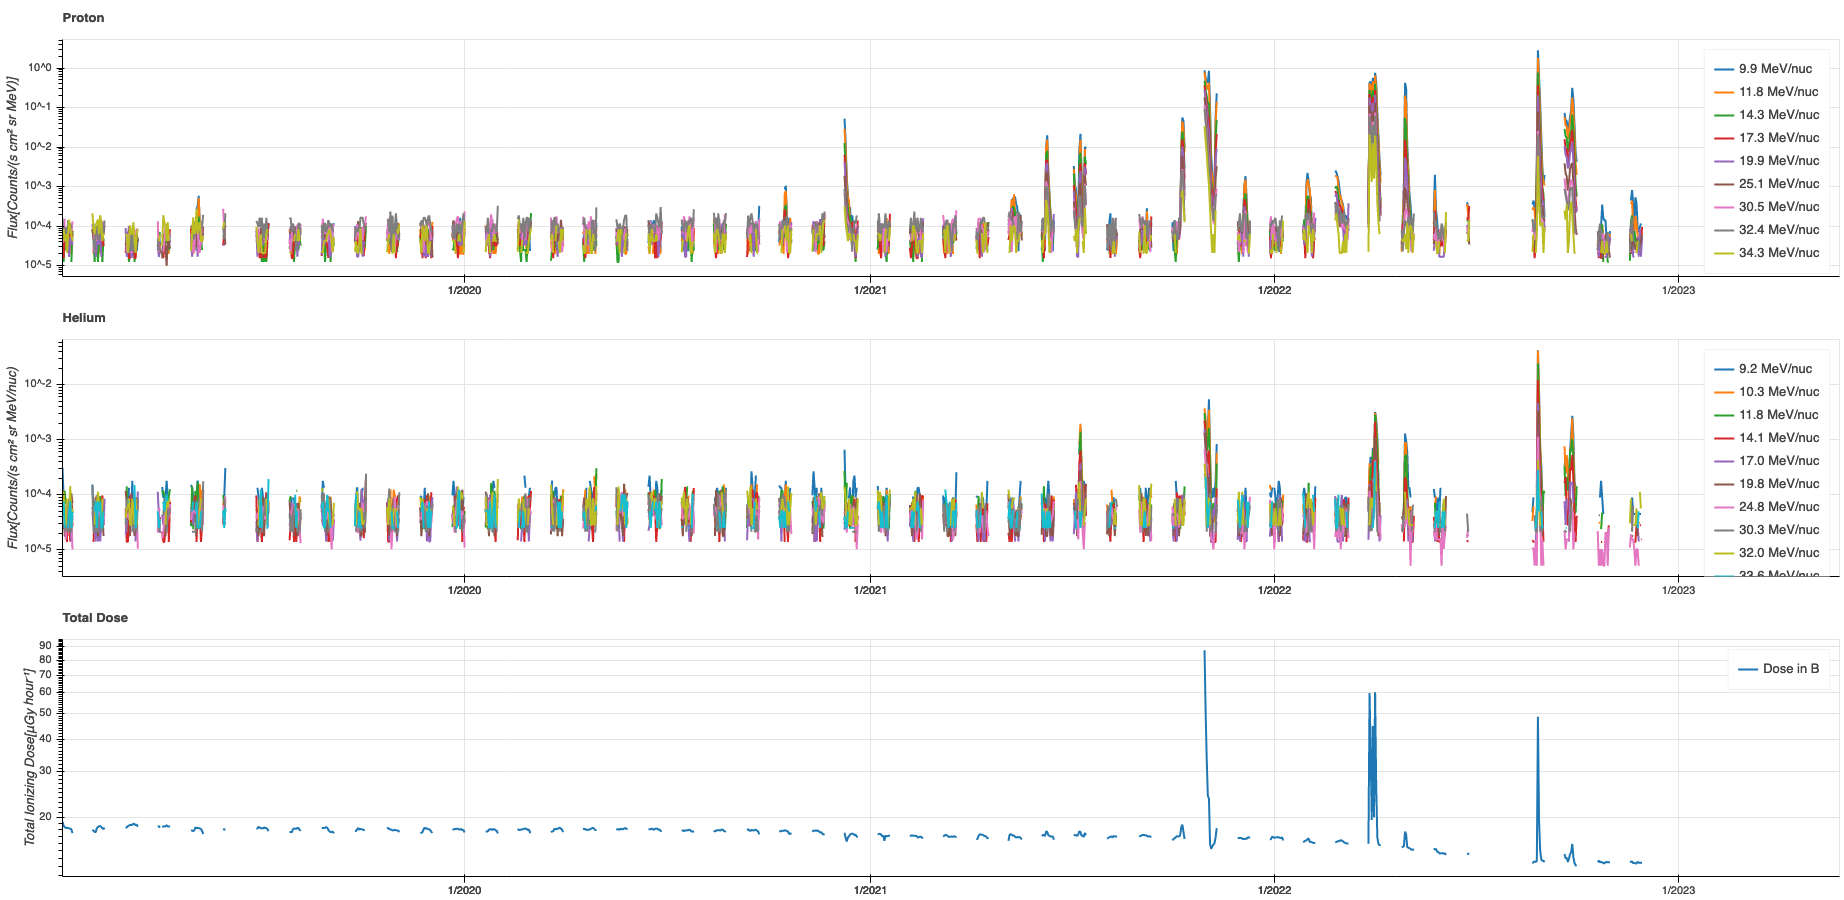
\includegraphics[angle = 90, width =\textwidth, height = \textheight]{images/LND-proton-helium-TID.png}
    \caption[The overview of proton, helium flux and \ac{TID} measured by \ac{LND}]{The proton, helium flux and \ac{TID} temporal variation from 2019 to Nov 29, 2022, measured by \ac{LND} on the lunar far-side surface}
    \label{Fig:appendix_LND_proton_helium_TID}
\end{figure}
\clearpage
The above figures are generated by the \ac{LND} webplotter which is a web application that is used to visualize the \ac{LND} data in a quick and fast way. 
Currently, the webplotter is running in the server named etsasa and only be available for the internal users.
The webplotter is written in Python and the source codes are available in the github repository \url{https://gitlab.physik.uni-kiel.de/LND/lnd_webplotter}.

The data gaps of \ac{LND} data appear periodically every lunar night due to the switch off of the lander and  the \ac{LND} instrument. The larger data gaps are periods when the lander conduct experiements. After 2021, the number of intense \ac{SEP} are increased. Some of them dramatically enhanced the \ac{TID} on the lunar far-side surface. It is worth noting the three consecutive \ac{SEP} events on the April of 2022, as shown in Fig.~\ref{Fig:appendix_LND_proton_helium_TID}. They occured shortly after \ac{LND} switched on and disappeared before the end of the lunar day. \ac{LND} obtained the completed proton, helium and \ac{TID} time profiled during these three \ac{SEP} events. Therefore, these three \ac{SEP} events provide a good opportunity to study the \acp{SEP} and its radiation impact on the lunar far-side surface.

In addition to the April 2022 events, there are other \ac{SEP} events, as shown in Fig.~\ref{Fig:appendix_LND_proton_helium_TID}, including the first \ac{SEP} event in May 2019 and the first \ac{GLE} event at the end of 2021, though not completed.

% create a table of SEP list that LND measured
\begin{table}[!tbhp]
    \centering
    \caption[\ac{LND} \ac{SEP} events lists]{A list of \ac{SEP} events observed by \ac{LND} between 2019 and 2022}
\begin{tabular}{cccccc}
    \hline
    No.     &  Start time    & End time      & Radiation  & Peak energy \\
            &                &               & hazard      & (Proton, MeV)\\
    \hline
    1       &   2019-05-04 12:00 & 05-06 00:00               & N  & $\sim$ 10\\
    2       &   2019-05-06 06:00 & 05-06 18:00              & N  & $\sim$ 20 \\
    3       &   2019-10-16 18:00 & 10-19 00:00             & N  & $\sim$ 20 \\
    4       &   2019-12-09 06:00 & 12-12 00:00             & N  & $>$ 35 \\    
    5       &   2021-06-09 06:00 & 06-12 00:00             & Y  & $>$ 35 \\
    6       &   2021-07-04 06:00 & 07-07 00:00             & N  & $>$ 35 \\
    7       &   2021-07-09 10:00 & 07-12 06:00             & Y  & $>$ 35 \\
    8       &   2021-07-13 12:00 & 07-15 06:00             & Y  & $>$ 35 \\
    9       &   2021-10-09 06:00 & 10-12 00:00             & Y  & $>$ 35 \\
    10      &   2021-10-30 08:00 & 11-06 05:00             & Y(intensive)  & $>$ 35\\
    11      &   2021-11-09 10:00 & 11-10 08:00             & Y  & $\sim$ 30 \\
    12      &   2021-12-05 05:00 & 12-07 09:00             & N  & $\sim$ 30 \\
    13      &   2022-01-29 22:00 & 02-03 11:00             & N  & $\sim$ 30 \\
    14      &   2022-02-25 06:00 & 03-01 19:00             & N  & $\sim$ 30 \\
    15(a,b,c) & 2022-03-28 06:00 & 04-07 01:00             & Y(intensive)  & $>$ 35 \\
    16      &    2022-04-28 00:00 & 05-04 06:00             & Y  & $\sim$ 30 \\
    17      &   2022-05-25 16:00 & 05-26 23:00             & N  & $\sim$ 20\\
    18      &   2022-08-26 08:00 & 09-01 11:00             & Y(intensive)  & $>$ 35 \\
    19      &   2022-09-19 23:00 & 09-39 00:00             & Y  & $\sim$ 30 \\
    20      &   2022-11-19 10:00 & 11-20 10:00             & N  & $\sim$ 15 \\
    \hline
\end{tabular}
\label{Tab:appendix_LND_SEP_list}
\end{table}

The start time and end time are determined by the eye and have larger uncertainty. 



\section{Housekeeping data of \ac{LND}}

Below

\ac{LND} has six temperature measusment sensors, monitoring the temperature variation of the \ac{SH} and the \ac{EB}. Two temperature sensors are fixed near the \acp{SSD}, one inside of the \ac{EB}, and the remain three are fixed on the power board, the analog board as well the digital board. The time variations of temperature are given in the panel (a) of Fig.\ref{Fig:appendix_LND_Housekeeping}. Like
 
The temperature sensor only operates together with LND on the day time. 
The temperature variation on the lunar surface

\begin{figure}[!htb]
    \centering
    \subfloat[]{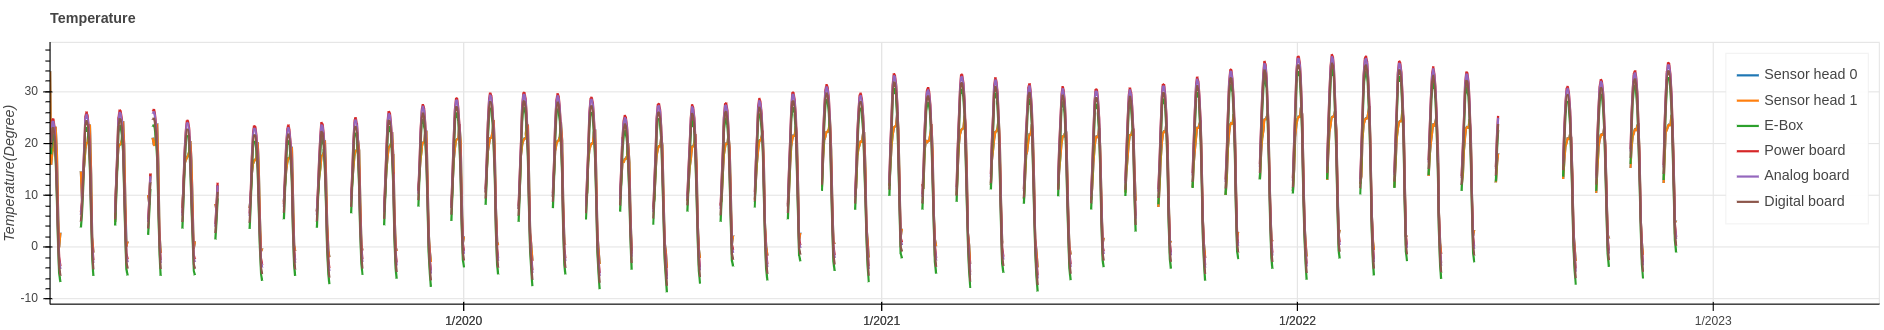
\includegraphics[angle =  90, width = 0.34\textwidth, height = 0.9\textheight]{images/lnd_temperature.png}}
    \subfloat[]{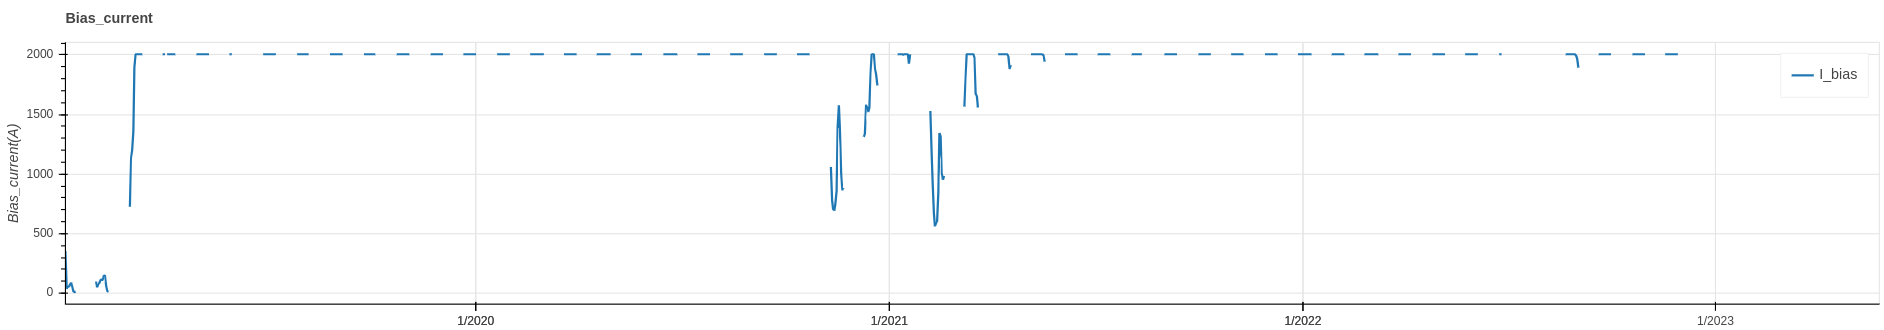
\includegraphics[angle = 90, width = 0.33\textwidth, height = 0.9\textheight]{images/lnd_bias_current.png}}
    \subfloat[]{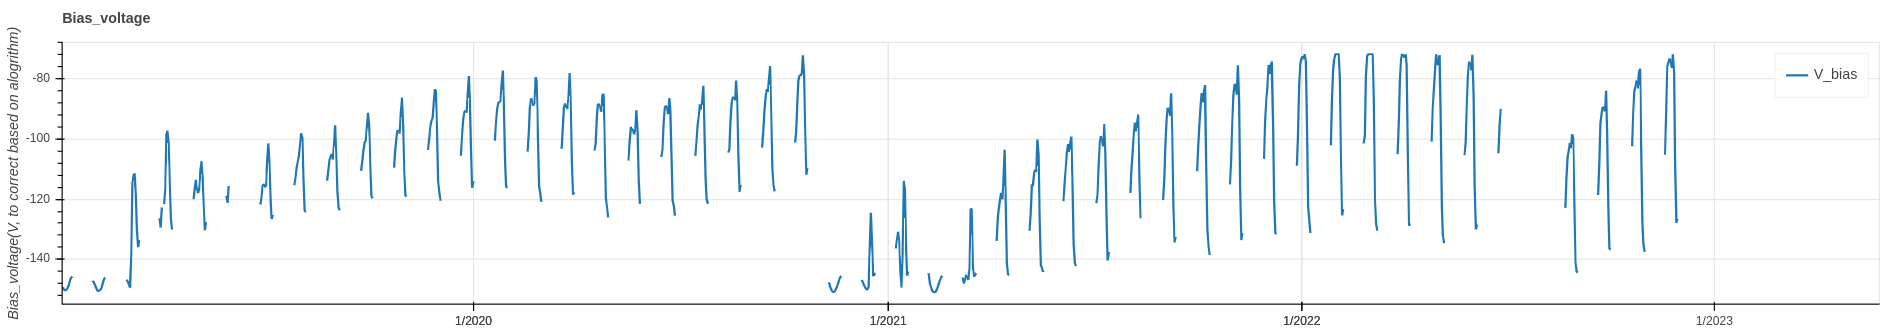
\includegraphics[angle = 90, width = 0.33\textwidth, height = 0.9\textheight]{images/lnd_bias_voltage.png}}
    \caption[LND temperature, bias current, and bias voltage variations]{The variation of housekeeping data including (a) temperature, (b) bias current, and (c) bias voltage. The temperatures are measured by the sensors assembled inside of LND sensor head and electronic box. The overview plot  2019 to Nov 29, 2022. }
    \label{Fig:appendix_LND_Housekeeping}
\end{figure}

\section{Correction of the LND bias current and voltage}

Due to the noise of the detectors, the bias current reach the limit of the meaurements at 2$\mu$A. 

Below are the scripts used to calculate the correct bias voltage and current that measured on the LND instrument from Stephan B\¨ottcher (private communication), who is the desinger of the LND instruement hardware and software in the IEAP.
\begin{lstlisting}[!htb]
# The Awk script for the LND bias current and voltage correction
# HK_Ibias and HK_Vbias are the bias current and voltage measured on the LND instrument
# HK_T_LVPS is the temperature of the LND instrument ( TODO: check the meaning of the LVPS)
# degC is the function to convert the temperature from Kelvin to Celsius
#================================
function Ibias() {
    a = $(HK_Ibias+3)
    if (a>4000) a = (147.3 + degC($(HK_T_LVPS+3))*0.164 - $(HK_Vbias+3)*0.05488) / 0.01810
    return a*0.4928
}

function Vbias() {
    return $(HK_Vbias+3)*0.05488 + $(HK_Ibias+3)*0.01810
}

\end{lstlisting}



\section{The change of LND data process pipeline}
\label{chp:appendix_LND_data_process_pipeline}

\section{Discrepanchy between LND and CREME}

\section{Heavy ion spectra}

\section{He3 spectra}
\label{chp:appendix_LND_He3_spectra}
Mostly the instrument effect, the He3 spectra is not reliable.

\section{L1 responce simulation}

